%!TEX root = ../physical-olympics-2.tex
\chapter{动力学}


\section{牛顿定律}

\subsection{概述}
中世纪到近代以来物理学的发展,\,可谓沧海桑田,\,旧的观点被否定,\,几十年以后突然又以全新的面貌出现在物理学理论中.\,其中,\,实验中观察到各种令人惊诧的结果,\,无论物理学所依托的数学形式一变再变,\,要说亘古不变的主题,\,恐怕只有自然界的神奇与深邃,\,和我等凡人难以参透其中奥妙却仍为之孜孜不倦研究的决心.\,物理是一门研究自然界存在的运动并提出解释与理解方法的学科.\,运动形式多种多样,\,变化万千,\,但很多都被我们或多或少地解释,\,其实总结来看,\,从古至今我们也仅仅拥有过两类解释:\,一类由牛顿提出,\,一类则来自爱因斯坦.\,前前后后经历了大概以下发展:

\begin{description}
	\item[亚里士多德:]\, 天体运行,\,自由落体是自然(nature)的运动;\, ``树欲静而风不止''是强迫(violent)的运动.\,但错误地认为``物体越重,\,下落越快''
	\item[伽利略:]\, 辩证地看待亚里士多德的观点,\,开创性地提出相对性原理,\,成功论证与形成惯性与常见运动的正确认识.
	\item[笛卡尔,\,惠更斯等:]\, 成功得到大量动力学公式,\,包括后来的牛顿第二定律,\,动能的表达式与能量守恒定律,
	\item[牛顿开创的相互作用观:] \, 开创性的提出物质间存在相互作用,\,相互作用是改变物质运动状态的原因.\,并很好地把天体的运动归结到互相之间产生的相互作用上.\,后人建立了场的理论以后,\,超距的粒子间相互作用就不再被理论学家们采纳了,\,而要理解为场与粒子的相互作用,\,再晚一点,\,场和粒子都被赋予了波粒二象性,\,粒子也要被理解为场,\,但所有场都要被被分解为平面波,\,平面波又要被量子化.\,如果没有相互作用,\,那么这些平面波的运动状态就不会发生改变,\,只有相互作用才会改变其运动,\,或传播方向发生偏折(发生散射),\,或强度发生改变(粒子的产生与湮灭).\,牛顿的观点是以\emph{相互作用}(interaction)为核心的观点.
	\item[拉格朗日,\,哈密顿等:]\, 将牛顿的结果与观点上升到\emph{分析力学}(analytic mechanics)的高度.\,将复杂体系的结构浓缩在统一的一个能量函数或作用量泛函数中.\,为后来场论建立和相对论,\,统计力学,\,量子力学的发展都提供了理论支持.
	\item[马赫:]\, 批判牛顿的过于绝对的时空观.\,预言质量分布会对惯性本身产生影响.
	\item[爱因斯坦开创的几何观:] \,  仿佛又回到了亚里士多德,\,不仅仅是无相互作用下的匀速直线运动,\,一切在万有引力下的天体运动其实也是``自然''的运动.\,看上去复杂的曲线运动不过也是沿对被引力所扭曲的弯曲时空几何下的天然``直线''---测地线(geodesic)运动而已.\,对引力问题提出开创性的解释.\,率先描绘了20世纪建立的若干理论的物理图像.
	\item[天体物理,\,粒子物理:]\, 爱因斯坦以后的理论研究中很多问题还处于开放状态.\,时而采用牛顿的相互作用观,\,时而采用爱因斯坦的几何观.\,是一种两个图像的有机结合.
\end{description}

我们今天说\emph{经典力学}(classical mechanics)大多数情况即指\emph{牛顿力学}(Newtonian mechanics),\,指的是由伽利略最初引领,\,笛卡尔,\,惠更斯等奠基,\,牛顿集大成的一套理论.\,它以伽利略的\emph{两种新科学的对话与数学展示}(Discorsi e dimostrazioni matematiche intorno a due nuove scienze)和牛顿的\emph{自然哲学的数学原理}(Philosophi\ae\ Naturalis Principia Mathematica)两篇文献为核心.\,逻辑上以质点的牛顿三大定律为基础.\,不包括后来上升到的分析力学层次,\,作为绝对时空观适用伽利略变换,\,不兼容相对论.

牛顿定律总结如下:
\vspace{0.5cm}

\hrule
\begin{enumerate}
	\item 第一定律:\quad 在惯性系中,\,一个质点应静止或匀速直线运动.\,除非有外力施加于物体.
	\item 第二定律:\quad 在惯性系中,\,质点受力的矢量和$\bs{F}$等于其质量$m$与加速度$\bs{a}$的乘积.
	\item 第三定律:\quad 一个质点对另一个质点施加作用力时,\,另一个质点同时将施加反作用力于第一个质点,\,作用力与反作用力等大反向共线.
\end{enumerate}
\hrule
\vspace{0.5cm}

三个定律之间的联系是很值得讨论的.\,对三个基本定律的设置反映了很多物理思想\footnote{例如爱因斯坦狭义相对论的两个假设在某种意义上与牛顿第一第二定律的逻辑完全一致.\,都是先定义时空背景再阐述物理规律的共性.}.\,分析如下:

\subsection{牛顿第一定律}
牛顿第一定律旨在阐述时空的平直性.

也正基于以上这一点,\,我们不能仍为牛顿第一定律可以由牛顿第二定律出发推导.\,它不是表面上的牛顿第二定律中$\bs{F}=\bs{0},\,\bs{a}=\bs{0}$的特例.\,恰恰相反,\,即使从形式上看,\,也应当先由牛顿第一定律给出\emph{惯性系}(inertial frame)的概念才能适用牛顿第二定律.\,那么怎样的参考系是惯性系呢?\,牛顿第一定律是暗含认可\emph{绝对惯性系}(absolute inertial frame)的存在性的.\,在这样第一个系中牛顿第一定律才可以成立.\,这一个系无非就是由某种特殊运动状态的观察者(绝对观察者)建立的三维欧几里得空间坐标系外带一维时间坐标.\,而只要质点不受力(力是对相互作用的描述,\,只要远离其它所有物质就会使质点成为\emph{孤立}(isolated)的),\,就会静止或匀速直线运动,\,所谓匀速直线运动是指:
\[\begin{pmatrix}x(t)\\y(t)\\z(t)\end{pmatrix}=\begin{pmatrix}x(0)\\y(0)\\z(0)\end{pmatrix}+\begin{pmatrix}v_x\\v_y\\v_z\end{pmatrix}\cdot t\]

其中三个速度$v_x,\,v_y,\,v_z$都是常数.\,但是我们发现,\,相对这个系做匀速直线运动的另一个无自转观察者建立的系中,\,原来做匀速直线运动的质点现在依然做匀速直线运动.\,所以这样的系也叫做惯性系,\,可以叫做相对惯性系.\,即:\,惯性系就是任何相对绝对惯性系做匀速直线平动的参考系.\,而惯性系就是牛顿定律成立的前提条件.

所以牛顿的经典力学体系的第一大特点是承认绝对惯性系的存在性.\,实际上承认这一点也几乎等价于承认了时空的平直性.\,只不过在众多彼此等价(任何物理实验都不足以判断这些系的不等价性)的系中,\,牛顿认为还应当有一个第一性的,\,``最初''的惯性系.

\subsection{牛顿第二定律}
牛顿第二定律是牛顿定律的核心,\,旨在描述相互作用对运动的影响.

\emph{相互作用}(interaction)是牛顿经典力学后经过了几百年发展而浓缩出来的更普遍的概念.\,如果没有相互作用,\,物质基本的运动模式就是``惯性''的,\,如匀速运动的粒子或传播的平面波.\,任何使物质偏离这种``惯性''运动的模式的原因就都在相互作用上.\,相互作用的模式是多种多样的,\,除了牛顿指出的下面仔细讨论的情形,\,光会因为与物质相互作用而产生吸收和散射,\,两个惰性气体原子靠近时两个电子云也会产生量子的诱导极化而使原子间产生范德瓦耳斯吸引.\,这些都是广义的相互作用,\,但是为了描述它们,\,前者需要借助波来描述光这种物质,\,后者还需要借助波函数来描述电子云,\,相互作用更是要依赖于薛定谔方程等来理解.\,所以经典物理理论有它的适用性,\,这一点在下面我们需要记住.

这也就是牛顿经典力学体系的第二大特点了:\,物质的基本模型一律视作\emph{质点}(mass point)\footnote{牛顿甚至认为光也适用于质点模型},\,相互作用的基本模型一律视作\emph{力}(force),\,质点具有惯性这一基本属性,\,用\emph{质量}(mass)来描述.

从牛顿第二定律$F=ma$形式上看,\,难免会由于数学思维得出``用力来定义质量的多少''或者是``用质量定义力的大小''这样的观点,\,而进入力与质量循环定义的误区.\,但实际上谁也没有定义谁.\,因为正常的物理思维是先要提前定义质量和力:

首先质量是受力物体所固有的属性之一,\,它具有广延性:\,如果把质量为$m_1$的质点与质量为$m_2$的质点复合为一个大质点,\,其质量变为$m_1+m_2$.\,可比性:\,任意两个质点的质量都可以依照在同样大小的力下的行为来比较其质量的比例关系\footnote{事实上用碰撞实验可以给出一个更简单的比较质量的方法,\,让待测质量的质点以一个单位的速度去正碰撞一个以$x$个单位速度运动的单位质量的质点,\,若恰好停下就说明待测质量为$x$个单位质量,\,若没停下就改变$x$的值直到停下.}.\,和固有性:\,只要质点没有变性,\,质量就不变,\,所以在不同参考系去看同一个质点,\,在运动的不同时刻质量都是严格不变的,\,也称``质量守恒'',\,我们将避免这一称呼,\,因为一般的守恒量只是针对一个参考系中的过程中的各个状态,\,而换一个系看守恒量往往要变,\,质量却显然不变,\,这是其一;\,另外相对论下质量就不再守恒了,\,它不普遍,\,这是其二.

力也是对固有的相互作用的强度做的描述.\,它也是固有的,\,应当有一种合理的公式去描述施力物体的状态如何影响施加的力(这个力也与受力物体的状态有关).\,而且如果换一个参考系考虑,\,力的强度是不变的.\,根据力对质点产生的效果,\,力也应当具有矢量性,\,不同两个力是可以比较的,\,很多情况下甚至可以叠加:\,多个施力物体互不影响各自施加的力,\,同时作用于同一个受力物体,\,在生活中这种现象非常常见,\,不难得出这样的总结.

于是才有了牛顿的著名论断:
\[\bs{F}=m\bs{a}\]

这样一个定律内容是丰富的,\,它首先是兼容于伽利略相对性原理从而自洽:\,在另外的惯性系中考察,\,$F$和$a$都是不变的.\,但是又不是兼容于相对性原理的唯一解决方案,\,狭义相对论,\,就提供了另一套可能性,\,在低速极限$v\ll c$时狭义相对论的动力学方程表达式和这并无二致;\,其次质量$m$作为系数联系了力(原因)与加速度(结果)这并不是偶然,\,它也是为了和叠加原理相协调:\,一份的力作用在一份质点上产生这样的加速度,\,那么把两份力各自作用在两份质点上那就还是产生同样的加速度.\,所以力除以质量决定运动学加速度\footnote{即$F/m=f(v,\,a)$}那是天经地义.\,至于为什么两份力作用在原来的一份质点上会产生加速度加倍的效果,\,这就是经典力学中的类似于公理性质的存在了.

\subsection{牛顿第三定律}
牛顿第三定律是对``相互作用''中的``相互性''的刻画,\,暗示了动量与角动量守恒.

任何物理理论,\,如果妄想在短短几条式子中道尽万千世界发展与变化的规律,\,都是玄学而不是科学.\,科学的精神是要基于事实,\,进行总结与归纳,\,借助数学进行基本的抽象与再创造.\,所以现实就是,\,世界的运行本就是复杂的,\,不可预测的.\,物理学的发展史也就充满了惊人的转折:\,每当人们以为在某一个大的领域有简单而清晰的图像共识的时候,\,总是会有意外发生告诉人们特殊情况下理论不再适用.\,原则上,\,没有任何命题能够成为物理学上的公理:\,它能无条件适用于从宇观到微观的方方面面.

牛顿清楚地意识到了物质与物质之间相互作用的复杂性,\,是不可能用几个简单的公式写出所有情况下他的理论中两个任意质点之间的作用力的.\,所以退而求其次,\,用牛顿第三定律来描述了所有情形下这样的力需要满足的条件.\,的确合情合理.\,但是又看牛顿第三定律的提法本身是否合理?

实际上我们先注意到动量守恒和角动量守恒的条件比牛顿第三定律的条件要强(也更本质):\,我们可以由前者推导出后者.\,以动量为例,\,动量是用来描述一个体系的动力学运动趋势的.\,动量守恒就意味着,\,如果一个孤立的体系的一部分``平均地''在初始时刻具有向前运动的趋势,\,比如一部分向前运动而另一部分静止.\,那么之后就绝对不可能演化为向后运动.\,或者还可以这么理解:\,如果看到一个质点在做一个非匀速直线运动:\,比如忽快忽慢的直线运动,\,那么显然单独看质点本身动量并不守恒.\,但是这必然意味着质点不是孤立的,\,必须和别的体系一同看作一个整体,\,质点增加或减少的动量必须由体系的另一部分的动量减少或增加来抵消,\,来满足整体动量守恒的需求.\,如果体系仅仅由两个质点构成,\,再把动量的增加或减少的快慢理解为受力(动量定理),\,我们就有了牛顿第三定律中关于相互作用力等大,\,反向的部分.

所以动量守恒可以用来``证明''牛顿第三定律中的一对相互作用力.\,同理角动量守恒则可以用来证明牛顿第三定律中质点间相互作用力共线的部分.\,最后读者可以验证牛顿第三定律的数学形式为\footnote{$\bs{F}_{12}$表示1给2的力.}:
\[\bs{F}_{12}+\bs{F}_{21}=\bs{0}\quad,\quad \bs{r}_2\times\bs{F}_{12}+\bs{r}_1\times\bs{F}_{21}=\bs{0}\]

之所以这么理解是因为,\,动量守恒和角动量守恒显得更普适.\,事实上,\,它们是体系物理规律在空间平移对称性和旋转对称性下具有协变形式的直接推论.\,这一点是由近代著名的\emph{诺尔特定理}(Noether Theorem)这一数学定理精确证明了的.

也正是牛顿第三定律暗示了牛顿经典力学体系的缺点.\,因为我们无法解释牛顿第三定律的``自然性'',\,取消牛顿第三定律所构成的体系无非是具有外力的非孤立系(动量不守恒),\,牛顿第三定律为体系增添的``结构性要求''并没有很好地由理论解释与包含.\,所以才有了后来建立在对守恒量,\,尤其是能量进行强调的分析力学理论的提出.

\subsection{质点系与它的牛顿定律}
对于复杂体系,\,牛顿提出一种可能的等效观点,\,就是把任意这样的体系看做是一种离散的质点系的推广.\,质点系由质点集合$\{(m_i,\,\bs{r}_i)\},\,(i=1,\,2\,\cdots \,n)$组成.\,我们只要找到从质点理论到有限质点构成的质点系理论中那些不变的结论,\,就有理由相信这些结论可以推广到复杂的真实体系.\,因为真实体系被期待可以用一个足够大数目的质点系来近似.\,对于复杂的质点系首先需要引入\emph{质心}(center of mass,\,{\rm CM})的概念:
\[\overline{\{(m_i,\,\bs{r}_i)\}}=(m_C,\,\bs{r}_C)\]

我们的做法是:\,直接把质心理解为一个新的质点,\,它具有新的质量$m_C$和位置$\bs{r}_C$,\,并满足表达式:
\[m_C=\sum_i m_i\quad;\quad \bs{r}_C=\frac{\sum_i m_i\bs{r}_i}{\sum_i m_i}\]

可以把上式读作:\,质心的质量等于质点系的总质量,\,质心的位矢是各个质点位矢关于质量的加权平均.

质心的求法是符合交换律与结合律的.\,这在质量上是显然的,\,因为质心质量就是各个质点质量构成的连加式.\,对于质心位矢,\,考虑总质量为$m_1$的第一个质点系$(m_{1i},\,\bs{r}_{1i})$和总质量为$m_2$的第二个质点系$(m_{2j},\,\bs{r}_{2j})$复合而成的整个质点系,\,如果直接算两个体系质心形成的质心:
\[\frac{m_1\bs{r}_{1C}+m_2\bs{r}_{2C}}{m_1+m_2}=\frac{\displaystyle\sum_i m_{1i}\cdot \frac{\displaystyle\sum_{i} m_{1i}\bs{r}_{1i}}{\displaystyle\sum_i m_{1i}}+\displaystyle\sum_j m_{2j}\cdot\frac{\displaystyle\sum_{j} m_{2j}\bs{r}_{2j}}{\displaystyle\sum_{j} m_{2j}}}{\displaystyle\sum_i m_{1i}+\displaystyle\sum_j m_{2j}}=\frac{\displaystyle\sum_{k\in 1\& 2}m_k\bs{r}_k}{\displaystyle\sum_{k\in 1\& 2}m_k}\]

可以发现这就是整个体系的质心.\,这种方法就是``组合法'',\,比如求几根棍子的质心,\,可以把棍子替换为在质心的质点再求.\,由此还可以引申出``割补法''或者``负质量法'',\,不过就是把上式反过来理解:\,如果我们要求第一个体系的质心,\,不难验证可以这样求:
\[\bs{r}_{1C}=\frac{m\bs{r}_C-m_2\bs{r}_{2C}}{m-m_2}\]

动态地看待求质心的式子,\,还可以发现,\,求导以后,\,我们得到了质心作为一个在运动的质点,\,其速度,\,加速度也是可以直接从原质点系来做加权平均的:
\[\bs{v}_C=\frac{\sum_i m_i\bs{v}_i}{\sum_i m_i}\quad;\quad \bs{a}_C=\frac{\sum_i m_i\bs{a}_i}{\sum_i m_i}\]

为了推导出质点系的类似的牛顿定律,\,我们发现牛顿三大定律是缺一不可的.\,当然原则上如果没有牛顿第三定律,\,我们就把作用在每一个质点$m_i$上的合力,\,不管施力物体是谁,\,记作$\phantom{}^tF_i$,\,``t'' for ``total''.\,原则上我们也可以得到:
\[\phantom{}^t\bs{F}=\sum_i m_i\bs{a}_i\quad \phantom{}^t\bs{F}=\sum_i\phantom{}^t\bs{F}_i\]

这一点很容易证明,\,只需要把每个质点的牛顿定律加起来即可.\,但是注意到牛顿第三定律既然正确,\,我们就可以做进一步的研究:\,把任何质点受力分解为\emph{内力}(internal force)和\emph{外力}(external force):
\[\phantom{}^t\bs{F}_i=\phantom{}^{in}\bs{F}_i+\phantom{}^{ex}\bs{F}_i\]

内力指$i=1,\,2\,\cdots\,n$个质点之间一对一对存在的力,\,所以实际上不如写明:
\[\phantom{}^{in}\bs{F}_i=\sum_{j\neq i}\bs{F}_{ji}\]

最后单独的那个真正的外力以后直接简写为$\phantom{}^{ex}\bs{F}_i=\bs{F}_i$.

经过这么一番折腾完以后,\,我们还是把所有质点的牛顿定律来求和,\,但是注意到由于牛顿第三定律关于相互作用力等大反向的部分,\,内力相互抵消,\,得到:
\[\bs{F}=\sum_i m_i\bs{a}_i\quad \bs{F}=\sum_i \bs{F}_i\]

这就是质点系的牛顿第二定律,\,相比上面那个也对的直接把每个牛二加起来的表达式,\,能引起注意的变化只有一点,\,那就是:\,不需要考虑内力!\,但正是这一点极大地简化了很多实际问题的分析.

值得一提,\,我们顺理成章地要考虑另外两个层面的规律,\,一是``对质心'',\,二是``相对质心''.\,前者值的是,\,把质心作为一个质点来研究问题.\,那么问题也很简单,\,利用之前证明过的:
\[\bs{a}_C=\frac{\sum_i m_i\bs{a}_i}{\sum_i m_i}\quad \Rightarrow \quad m_C\bs{a}_C=\sum_i m_i\bs{a}_i\]

就可以得到:
\[\bs{F}=m_C\bs{a}_C\]

这就是著名的\emph{质心运动定律}(motion law of {\rm CM}).\,特殊的,\,如果合外力$\bs{F}=\bs{0}$.\,那么退化到\emph{质心守恒}:\,质心做匀速直线运动或者静止.

最后我们提出质心系的概念.\,\emph{质心系}(frame relative to {\rm CM})指:\,原点在质心的平动欧几里得坐标系.\,结合我们已经学过的和将来要学的所有内容我们把其性质罗列如下,\,请读者能够给出证明的直接证明,\,给不出的带着问题往下学习:
\begin{itemize}
	\item 质心系虽然有非惯性力,\,但非惯性力与原力系主矢和为零.
	\item 质心系虽然有非惯性力,\,但非惯性力系对质心的主矩为零.
	\item 质心系是零动量系.
	\item 质心系虽然有非惯性力,\,但非惯性力在过程中总功和为零.
	\item 取质心为原点能使质点系二阶矩最小,\,故刚体相对所有平行轴中以过质心的轴转动惯量最小.
	\item 只有取质心才能写出柯尼希定理.
\end{itemize}

\subsection{非惯性系的处理}
虽然牛顿定律只在惯性系中成立.\,但是如果我们选取一个相对惯性系的转动系,\,其原点速度加速度为$\bs{v}_C$与$\bs{a}_C$.\,而角速度与角加速度分别为$\bs{\omega}$与$\bs{\beta}$.\,本来在原来的惯性系中研究一个质点,\,正确的式子是:
\[\bs{F}=m\bs{a}\]

现在换了参考系以后,\,将不能仿照上式写出一个依然正确的式子.\,但是加速度变换总是对的:
\[\bs{a}=\bs{a}_C+\bs{\beta}\times\bs{r}'+\bs{\omega}\times(\bs{\omega}\times\bs{r}')+2\bs{\omega}\times\bs{v}'+\bs{a}'\]

而我们也永远认为力矢量在参考系变化下是大小与方向都不变的:
\[\bs{F}=\bs{F}'\]

代入就足以得到依然正确的,\,仅仅用新的非惯性系中的各个参量表示的类牛顿定律.\,我们以后将直接叫做非惯性系中的牛顿定律:
\[\bs{F}'+(-m\bs{a}_C)+(-m\bs{\beta}\times\bs{r}')+[-m\bs{\omega}\times(\bs{\omega}\times\bs{r}')]+(-2m\bs{\omega}\times\bs{v}')=m\bs{a}'\]

可以发现,\,这类似于需要为质点运动虚构一些力,\,它们全都称作\emph{惯性力}(force of inertial).\,包括:
\begin{itemize}
	\item 平动惯性力$-m\bs{a}_C$,\,典型的情况就是平动而非转动的非惯性系中的惯性力.\,特点是一个恒力,\,而与质点的运动状态无关.
	\item 切向惯性力$-m\bs{\beta}\times\bs{r}'$与惯性离心力$-m\bs{\omega}\times(\bs{\omega}\times\bs{r}')$,\,典型的情况是绕轴做旋转的参考系.\,特点是这两个力仅仅依赖于质点的位置,\,离轴越远力越大,\,在轴上力就消失了.
	\item 柯里奥利力$-2m\bs{\omega}\times\bs{v}'$,\,典型的情况是相对转动系还有运动的情况.\,特点是给出一个与位置无关,\,但是正比与速度大小,\,方向始终垂直于速度方向的力.
\end{itemize}

如果我们的研究对象是一个刚体而非质点,\,那么相当于每一个质点上都要受到不同的惯性力.\,此时如果考虑这些所有力作用在刚体上的等效合力和力矩,\,那么将是一个非常复杂的情况,\,尤其是,\,各个柯里奥利力将对刚体整体造成所谓的``回转力矩'',\,用这个观点可以解释很多第七章刚体中的现象,\,感兴趣的读者可以参考相关资料.

\section{动量定律}
这四节我们将罗列质点与质点系动力学的核心内容.\,读者应当具有初等的牛顿理论的基础.\,这一部分与三个牛顿定律的关系如何?\,首先它们是牛顿定律的自然延伸,\,属于并占据经典力学的主要部分.\,其次这些结论与相关推论适用性很强.\,比如三个守恒律:\,动量能量与角动量的守恒几乎是在所有物理理论中普适的.\,从内容上看关于质点系的定律自然就包含了单质点的相应特殊情况.\,而写法总是有三种:\,相对地面系的,\,相对质心系的和把质心作为质点的.\,联系三种写法的是质心系独有的各个柯尼希定理.\,最后,\,能量比较特殊我们单独列一小节多加阐述,\,具体的碰撞问题加一节,\,最后再补充一个新的位力定律.\,便构成了一$3\times3$条定律为主干的本章的内容.\,实际上也就是牛顿经典力学的核心部分.

\subsection{质点的动量}
质点的\emph{动量}(momentum)定义为:
\[\bs{p}=m\bs{v}\]

很直接地可以推导出质点的\emph{动量定理}(law of momentum)来,\,用$\bs{F}$表示合力:
\[\bs{F}=\frac{\ud \bs{p}}{\ud t}\]

证明过程就是把牛顿定律右侧拿来等量代换.

质点动量守恒并不是守恒律最常见的提法.\,但是不管怎样,\,我们能看出来,\,如果在某方向\footnote{必须是直角坐标!\,比如极坐标下$F_\theta=0$但$p_\theta$不守恒,\,$L=rp_\theta$才是对应的守恒量,\,个中缘由涉及到分析力学.}分力为零,\,那么该方向分动量导数为零,\,从而是一个不变量.

\subsection{质点系的动量}
依据上一节的符号约定,\,质点系$\{m_i,\,\bs{r}_i\}$中第$i$个质点的牛顿定律写作:
\[\bs{F}_i+\sum_{j\neq i}\bs{F}_{ji}=m_i\bs{a}_i\]

所谓质点系的动量定理,\,无非就是把上式拿去对每一个质点求和,\,然后等号右侧化为动量的形式.\,过程中我们发现需要定义:

质点系的总动量:
\[\bs{p}=\sum_i \bs{p}_i=\sum_i m_i\bs{v}_i\]

外力矢量和:
\[\bs{F}=\sum_i \bs{F}_i\]

过程中内力全然抵消,\,这就导致了最后表达式简单地为:
\[\bs{F}=\frac{\ud \bs{p}}{\ud t}\]

\vspace{0.5cm}

接下来就是研究质心的两个层次,\,一是把质心作为质点研究等号左侧的``作用''和等号右侧的``动力学量'';\,二是考虑相对质心系的引入惯性力以后的新写法.

如果在地面系中质点系受到一个力$\bs{F}_\alpha$,\,那么把这个力移动到质心上以后,\,我们认为这个力是不需要改变的.\,但是如果考虑相对质心系,\,固然原来的力也是存在且不变,\,但是还得考虑惯性力.\,那么总的合力推导出来应当是:
\[\bs{F}_C=\bs{F}\quad ,\quad \bs{F}'=\bs{0}\]

后者是因为惯性力的合力$\displaystyle\sum_i -m_i\bs{a}_C=\sum_i -m_i\bs{a}_i=-\bs{F}$.\,我们发现有:
\[\bs{F}=\bs{F}_C+\bs{F}'\]

形如上式的式子都可以叫做\emph{柯尼希定理}(K\"onig theorem).\,再来看动量,\,质心动量就应当是质点系总动量,\,而相对质心系动量必然为零:
\[\bs{p}_C=\bs{p}\quad,\quad \bs{p}'=\bs{0}\]

前者由于质心的定义很容易看出来,\,后者一般被叫做:\,质心系是零动量系,\,两者之和符合:
\[\bs{p}=\bs{p}_C+\bs{p}'\]

这就不难看出:
\[\bs{F}_C=\frac{\ud \bs{p}_C}{\ud t}\]
\[\bs{F}'=\frac{\ud \bs{p}'}{\ud t}\]

最后我们讨论普遍的\emph{动量守恒}(conservation of momentum).

第一,\,动量守恒是普遍的,\,虽然表面上看$\bs{F}=\dfrac{\ud\bs{p}}{\ud t}$一个体系的动量只要外力不为零就会有非零的导数.\,但是根据动量守恒的精神,\,一个体系的动量增必然以另一个体系动量的减为代价,\,也就是需要注意到既然存在外力$\bs{F}$,\,那就需要考虑力作用的相互性.\,只要把所有施力物体都归入同一个体系使相互作用封闭.\,那么等号左侧只能是零,\,那么等号右侧就会有普遍的动量守恒.

第二,\,有些场合动量不以质点为载体而是以场为载体.\,动量依然守恒,\,毕竟我们将认为场给质点的力与``质点给场的力''构成反作用力符合牛顿第三定律.\,事实上只要可能涉及到超距作用就一定是要用场来处理的,\,不用场处理可能导致不精确甚至谬误的结果,\,这是因为牛顿第三定律都不一定适用.\,只要想想一个质点位置突然改变,\,由于相互作用传递速度必然有限导致相隔一定距离的第二个质点受力变化将会延迟,\,就不能使得这个力等于同一时刻的反作用力,\,那么两质点的动量和就不再守恒.\,另一种典型的情况是两个电流元之间的磁场安培力也不符合牛顿第三定律,\,全都是因为有场的动量未计入计算的缘故.\,所以这些场合,\,如果牛顿第三定律``近似''适用,\,我们才说质点系的动量``近似''守恒.\,严格的动量守恒设计场论的知识,\,有兴趣的读者可以进行相关学习.


\section{角动量定律}

角动量的逻辑与上一节是完全一致的.\,只不过在牛顿定律的数学处理上要多一步罢了.

\subsection{质点的角动量}
选取一个参考系的原点$O$以后便可以写出质点的位矢$\bs{r}$.\,那么质点受力对$O$的\emph{力矩}(moment of force,  moment, torque)定义为:
\[\bs{M}=\bs{r}\times\bs{F}\]

而为质点则定义一个动力学量也就是\emph{角动量}(angular momentum):
\[\bs{L}=\bs{r}\times \bs{p}=\bs{r}\times m\bs{v}\]

之所以这么做,\,一种想法是对牛顿定律$\bs{F}=m\bs{a}$两侧用$\bs{r}$叉乘的一种可能的构造思路\footnote{Noether定理才是严谨的构造思维.}.\,这就能给出\emph{角动量定律}(law of angular momentum):
\[\bs{M}=\frac{\ud \bs{L}}{\ud t}\]

证明过程只消注意到右边莱布尼茨法则出来两项的另一项$\dot{\bs{r}}\times\bs{v}=\bs{v}\times\bs{v}=\bs{0}$.

角动量定律有一个值得注意的点,\,那就是\emph{矩}(moment)的中心的选取的任意性.\,角动量(动量的矩)和力矩都因为是$O$点计算的才具有位矢$\bs{r}$,\,这个点叫做\emph{矩心}(center of moment).\,而选取不同的矩心的结果就会产生不一样的定律的表达式形式,\,它们都是对的.\,但是解题时何以选取?\,这个复杂的问题我们下一章再做简要介绍.

另一个点是原则上必须选取不动的点作为矩心.\,选取动点暗含两层意思,\,一是,\,可能需要把每一个粒子对动点的动量理解为相对速度对应的动量.\,二是,\,可能在求角动量的导数时要求的是跟随动点的角动量的导数.\,无论哪一点都将使得相应结论不再正确.\,当然,\,如果两种可能的更改都没有发生,\,即,\,仅仅是这一时刻对这一点列瞬时的角动量定律,\,下一时刻换下一个点列.\,那么这就是构成一个时时刻刻都成立的等式,\,只有在这种意义下角动量定律才可以原封不动地应用.\,否则需要重新从牛顿定律出发加以推导.

质点的角动量守恒也不是一个典型的结论.\,但是有一种典型的情形:\,就是平面上一个有心力作用下的质点运动是角动量总是守恒的.\,因为此时$\bs{F}\parallel \bs{r}\;\Rightarrow\;\bs{M}=\bs{0}$.

\subsection{质点系的角动量}

定义质点系的总角动量:
\[\bs{L}=\sum_i\bs{L}_i=\sum_i\bs{r}_i\times m_i\bs{v}_i\]

外力力矩和(不需要包括内力):
\[\bs{M}=\sum_i\bs{M}_i=\sum_i \bs{r}_i\times\bs{F}_i\]

每一个质点的牛顿定律,\,现在我们用每一个质点的位矢做叉乘:
\[\bs{r}_i\times\bs{F}_i+\bs{r}_i\times\sum_{j\neq i}\bs{F}_{ji}=\bs{r}_i\times m_i\bs{a}_i\]

然后再来求和,\,注意到牛顿第三定律中的``共线''性$\bs{r}_i\times \bs{F}_{ji}+\bs{r}_j\times \bs{F}_{ij}=\bs{0}$让第二项内力也一对一对抵消了.\,于是得到质点系的角动量定律:
\[\bs{M}=\frac{\ud \bs{L}}{\ud t}\]

\vspace{0.5cm}

同理,\,考虑把外力移动到质心形成的总力矩和相对质心系的力矩,\,把从质心出发的各个质点的位矢记作$\bs{r}_i'$,\,就有:
\[\bs{M}_C=\bs{r}_C\times \bs{F}\quad,\quad \bs{M}'=\sum_i \bs{r}_i'\times \bs{F}_i\]

后一个式子隐藏着一个关键信息:\,质心系中惯性力以质心为矩心时力矩和为零,\,这可以如下推导:
\[\sum_i \bs{r}_i'\times (-m_i \bs{a}_C)=-\left(\sum_i m_i \bs{r}_i'\right)\times \bs{a}_C=-\bs{0}\times \bs{a}_C\]

而质心的角动量与相对质心的总角动量为:
\[\bs{L}_C=\bs{r}_C\times m_C\bs{v}_C\quad,\quad \bs{L}'=\sum_i \bs{r}_i'\times m_i\bs{v}_i'\]

注意后一式中由于换系,\,相对质心速度应当为$\bs{v}_i'=\bs{v}_i-\bs{v}_C$.\,如此定义以后依然可以符合柯尼希定理:
\[\bs{M}=\bs{M}_C+\bs{M}'\]
\[\bs{L}=\bs{L}_C+\bs{L}'\]

对于后者我们简略写出证明过程:
\begin{align*}
	\bs{L}=\sum_i\bs{r}_i\times m_i\bs{v}_i &=\sum_i(\bs{r}_C+\bs{r}_i')\times m_i(\bs{v}_C+\bs{v}_i')\\
					 &=\bs{r}_C\times\left(\sum_i m_i\right)\bs{v}_C+\left(\sum_i m_i\bs{r}_i'\right)\times\bs{v}_C+\bs{r}_C\times\left(\sum_i m_i\bs{v}_i'\right)+\sum_i \bs{r}_i'\times m_i\bs{v}_i'\\
					 &=\bs{L}_C+\bs{0}+\bs{0}+\bs{L}'
\end{align*}

于是也就有质心的角动量定律和相对质心的角动量定律:
\[\bs{M}_C=\frac{\ud \bs{L}_C}{\ud t}\]
\[\bs{M}'=\frac{\ud \bs{L}'}{\ud t}\]

容易看出\emph{角动量守恒}(conservation of angular momentum)也是普遍的.\,而场的角动量也是可能涉及超距作用时需要考虑的因素.

\section{能量定律}
能量的情况就有一些不一样了.\,在动能定理的层面上逻辑相似,\,但是内力不再可以忽略,\,而且动能往往不守恒,\,即使守恒也不普遍,\,能量普遍地需要守恒,\,但这又不能在经典力学框架下加以证明.\,纯属特殊情况下的特殊结论或是一种令人信服的归纳假设.

\subsection{质点的动能}
力作用在质点上对质点做\emph{功}(work)的\emph{功率}(power)定义为:
\[P=\bs{F}\cdot\bs{v}\]

一个具体的过程才可以说做功,\,它等于功率的时间积分,\,也可以按照力点乘位移来做积分:
\[W_{1\rightarrow 2}=\int_{t_1}^{t_2}P\ud t=\int_{t_1}^{t_2}\bs{F}\cdot\bs{v}\ud t=\int_{t_1}^{t_2}\bs{F}\cdot\ud \bs{r}\]

质点的\emph{动能}(kinetic energy)则定义为:
\[T=\frac{1}{2}mv^2\]

这么定义的出发点也可以是从$\bs{F}=m\bs{a}$出发,\,两变同时点乘$\bs{v}$得到所谓的\emph{动能定律}(law of kinetic energy):
\[P=\frac{\ud T}{\ud t}\]

证明过程只需要注意到$\ud(\bs{v}\cdot\bs{v})=\ud(v^2)=2\bs{v}\cdot \bs{v}=2v\ud v$为恒等式.

质点动能守恒也不是一个典型的结论.\,如果质点受的合力始终垂直于质点速度,\,那么便有动能守恒.\,比如把质点约束在一个光滑的椭球面上做惯性运动,\,或者是让电荷在一个任意的不随时间变化的磁场中运动都属于这种情况,\,动能是不变量.

\subsection{质点系的动能}
定义质点系的总动能:
\[T=\sum_iT_i=\sum_i \frac{1}{2}m_i v_i^2\]

但是,\,单独求外力的功率和是没有用的,\,因为内力也有它的功率,\,且不为零.\,所以我们写出整个体系的总作用力的功率:
\[P=\sum_i P_i+\sum_{\{ij\}}P_{\{ij\}}=\sum_i \bs{F}_i\cdot \bs{v}_i+\sum_{\{ij\}}(\bs{F}_{ij}\cdot \bs{v}_j+\bs{F}_{ji}\cdot \bs{v}_i)\]

顾名思义,\,求和$\displaystyle\sum_{\{ij\}}$意为对每一对力涉及的后面的向进行求和.\,每一项必然涉及到两个质点,\,选取好每一对质点以后就可以写出项来而不在乎选取的顺序.\,故如果共有$n$个质点的话一共最多会有$\dfrac{n(n-1)}{2}$对,\,事实上既然$ij$交换要求项本身又不会变,\,总是有:
\[\sum_{\{ij\}}=\sum_{i=2}^n\sum_{j=1}^{i-1}\]

这样对每一个质点的牛顿定律点乘质点的速度:
\[\bs{F}_i\cdot \bs{v}_i+\sum_{j\neq i}\bs{F}_{ji}\cdot \bs{v}_i=m_i\bs{a}_i\cdot\bs{v}_i\]

同理,\,求和可得质点系的动能定律:
\[P=\frac{\ud T}{\ud t}\]

同理,\,考虑外力移动到质心后对质心运动做功的功率和相对质心系的系统所有力的功率和:
\[P_C=\bs{F}\cdot\bs{v}_C\quad,\quad P'=\sum_i \bs{F}_i\cdot \bs{v}_i'+\sum_{\{ij\}}(\bs{F}_{ij}\cdot \bs{v}_j'+\bs{F}_{ji}\cdot \bs{v}_i)'\]

这里也隐藏着两点,\,一是作用在质心上的力又只需要考虑外力了,\,因为内力的和本来就是零.\,二是质心系中的惯性力又因为做功总是零而不需要写在第二个式子中了,\,也就是:
\[\sum_i (-m_i\bs{a}_C)\cdot \bs{v}_i'=-\left(\sum_im_i \bs{v}_i'\right)\cdot\bs{a}_C=-\bs{0}\cdot\bs{a}_C\]

而质心的动能和相对质心的总动能为:
\[T_C=\frac{1}{2}m_Cv_C^2\quad,\quad T'=\sum_i\frac{1}{2}m_iv_i'^2\]

如此定义以后将符合柯尼希定理:
\[P=P_C+P'\]
\[T=T_C+T'\]

证明过程请读者自己完成.\,同时,\,也有对质心的动能定律和相对质心的动能定律:
\[P_C=\frac{\ud T_C}{\ud t}\]
\[P'=\frac{\ud T'}{\ud t}\]

导致能量与角动量和动量不同的原因是,\,动能守恒绝对不是什么普遍结论,\,不仅不普遍而且还很罕见.\,能量才是普遍守恒的.\,我们细细比较其中区别:


\subsection{其它能量形式}

从表面上看,\,很容易观察出来,\,即使整个质点系已经囊括了全部的施力物体了,\,相互作用是封闭的,\,也就是每一个质点上都没有外力只有内力:
\[\bs{F}_i=\bs{0}\]

此时依然总功率可以不等于零:
\[P=\sum_{\{ij\}}P_{\{ij\}}=\frac{\ud T}{\ud t}\neq 0\]

从而还和动量,\,角动量那样的守恒律已经成为了妄谈.

从实质上看,\,我们对于动量定律角动量定律还有一种说法:
\[\bs{F}=\frac{\ud \bs{p}}{\ud t}\quad,\quad \bs{M}=\frac{\ud \bs{L}}{\ud t}\]

力,\,带来动量的转移;\,力矩,\,带来角动量的转移.\,但是同样的说法换到做功上就不合适了:\,的确,\,下式成立:
\[P=\frac{\ud T}{\ud t}\]

但是功率不能认为是动能的转移.\,的确,\,功率是能量的转移;\,也的确,\,功率就是单位时间变成的动能.\,但是它不一定来自动能.\,只需要设想两个带正电的小球相互排斥而获得速度,\,那么显然把其间的力视作相互作用力时,\,两小球的动能并不是互相转移的关系,\,而是都因为力做功而获得动能,\,这个动能来自下面要讲的势能,\,或者场的能量.

所以能量守恒这一论调,\,不像另外两个守恒律,\,至少是不能从牛顿定律中单独推导.\,但是只要上升到分析力学立刻就可以发现能量守恒是完整体系相互作用不显含时间(稳定体系)的结果.\,在经典层面上通过补充下面三个独立而正确的说法便可以使得能量守恒可以被证明出来.

\subsubsection{保守力}
保守力意为由势能函数描述的力.\,势能函数是至关重要的概念,\,为了确定一个体系的运动,\,原则上只需要给出势能函数和初始状态便可以完全求解了.\,复杂的体系之所以复杂,\,一是粒子数大,\,二是初始状态随机.\,但是各式各样的整体行为,\,往往就蕴藏在任意两个粒子的相互作用的形式中.\,而这个相互作用我们相信它总是保守的.

就是说,\,存在二体相互作用函数,\,也就是\emph{势能}(potential energy)函数$V$,\,如果两个粒子分别在$\bs{r}_1$和$\bs{r}_2$.\,势能应当只与位置有关(与速度加速度无关),\,也不能含有时间:
\[V=V(\bs{r}_1,\,\bs{r}_2)\]

而势能决定作用力:
\[\bs{F}_{12}=-\nabla_2V\quad,\quad\bs{F}_{21}=-\nabla_1V\]

如果能够找到这样的势能函数,\,那么就把这样的力叫做\emph{保守力}(conservative force).

如何理解以上的形式?\,它的等价的写法是:
\[F_{12x}=-\frac{\partial V}{\partial x_2}\quad ,\quad F_{12y}=-\frac{\partial V}{\partial y_2}\quad ,\quad F_{12z}=-\frac{\partial V}{\partial z_2}\]
\[F_{21x}=-\frac{\partial V}{\partial x_1}\quad ,\quad F_{21y}=-\frac{\partial V}{\partial y_1}\quad ,\quad F_{21z}=-\frac{\partial V}{\partial z_1}\]
\[\ud V=V(\bs{r}_1+\ud \bs{r}_1,\,\bs{r}_2+\ud \bs{r}_2)-V(\bs{r}_1,\,\bs{r}_2)=-\bs{F}_{12}\cdot \ud \bs{r}_2-\bs{F}_{21}\cdot \ud \bs{r}_1\]

那么首先这就提出了一个要求,\,由于相互作用力总是应当满足牛顿第三定律的,\,而且体系应当也具有对称性,\,那么势能函数必然只取决于两个质点的相对位矢,\,且与两个质点的相对位矢的方向没有关系,\,只能和其大小有关系,\,也就是说:
\[V=V(R)\quad,\quad R=|\bs{r}_1-\bs{r}_2|=\sqrt{(x_1-x_2)^2+(y-1-y_2)^2+(z_1-z_2)^2}\]

这自然就可以计算出:
\[\bs{F}_{12}=-\frac{\ud V}{\ud R}\bs{e}_{12}\quad ,\quad \bs{F}_{21}=-\frac{\ud V}{\ud R}\bs{e}_{21}\]

其中$\bs{e}_{12}$和$\bs{e}_{21}$分别代表1指向2和2指向1的单位矢量.

第二点是,\,在任一个元过程中,\,这一对相互作用内力做的功的和,\,一方面由于动能定律等于转化为1和2的总动能$\ud T$,\,另一方面还等于势能的减少:
\[\bs{F}_{12}\cdot \ud \bs{r}_2+\bs{F}_{21}\cdot \ud \bs{r}_1=-\ud V\]

这就造成了能量函数$H=T+V$的守恒:
\[\ud T=-\ud V\quad \Rightarrow \quad H|_t=H|_{t=0}=E\]

在更多情况中,\,我们让施力物体静止在固定点,\,但是施力物体亦是一个质点系而非质点,\,研究单个质点作为受力物体的运动.\,那么显然此时质点符合$\bs{F}=m\bs{a}$.\,但是质点依然受到所的合力还是一个保守力,\,只需要把它与各个施力物体的势能函数相加,\,整体作为这个质点位矢的一元函数即可:
\[\bs{F}(\bs{r})=-\nabla V(\bs{r})\]

总之,\,原则上可以用势能函数描述的力就是保守力.\,虽然从中文还是英文的名字来看,\,似乎暗示了只要能量守恒就应当视作保守力,\,但这是不恰当的.\,例如一个不随时间变化的磁场中一个电荷的运动,\,显然动能不随时间变化是个常数,\,但这绝对不意味着体系的势能函数为$V(\bs{r})=0$或常数.\,的确,\,这样能够使得``能量函数''$H=T+V$守恒到一个常数$E=T|_{t=0}$,\,但是这样的势能函数不能用来刻画磁场给质点的力:
\[q\bs{v}\times \bs{B}\neq -\nabla V\]

所以这个力不能用势能来描述,\,从而并不是保守力\footnote{其实在分析力学中如果引入磁矢势$\bs{A}$那么这个力可以作为$U=-q\bs{v}\cdot \bs{A}$的负梯度,\,这中含有速度的势能叫做广义势函数.\,但是即使可以定义势函数,\,习惯上依然不把这个力叫做保守力.\,因为可以验证此时动能与这个势能的和又不再守恒了.}.


\subsubsection{约束力}

从微观相互作用到宏观发生了很复杂的变化.\,但是很多情况下体系依然存在一个势函数.\,例如单摆的动能和势能就可以写为:
\[T=\frac{1}{2}ml^2\dot{\theta}^2\]
\[V=mgl(1-\cos\theta)\]
\[H(\theta,\,\dot{\theta})=T+V\]

显然,\,这里用的不再是摆球的位矢$\bs{r}$作为势能的坐标.\,而是换成了$\theta$这样的\emph{广义坐标}(generalized coordinates),\,对应的广义力$-\dfrac{\partial V}{\partial \theta}$实际上是一个力矩,\,把广义力乘广义坐标的微分实际上就是释放的势能.\,我们发现小球受到的力是重力和绳子的拉力,\,这个势能函数实际上就是只考虑了重力势能.\,为什么可以这么做?\,这是因为绳子的拉力就是一个十分典型的约束力.\,从守恒律的角度来看,\,它不会影响其他力造成的动能和势能和的守恒.\,这一点也十分自然,\,因为这样的绳只的确没有任何机制能够存储能量.

这也就是说,\,对\emph{约束力}(constraint force)的要求主要就体现在它不能做功上.\,显然,\,上一例中的绳子拉力并不对摆球做功.\,容易验证,\,光滑的面接触,\,不可伸长的轻绳轻杆连接的两个物体,\,其约束力对约束的单个物体多整个体系做的总功总会是零.\,它们都是典型的约束力.\,更详细的讨论见下一章.\,我们最后以一个例子来看待对约束力的要求.

如果一个体系的两个广义坐标$q_1,\,q_2$对应的物体之间有一个约束$F(q_1,\,q_2)=0$,\,如两个用长为$l$的不可伸长的轻杆连接的质点的$x$坐标就必须满足:
\[F(x_1,\,x_2)=(x_1-x_2)^2-[l^2-(y_1-y_2)^2-(z_1-z_2)^2]=0\]

那么在任何过程中两个坐标的变化量$\ud q_1$和$\ud q_2$就必须满足:
\[\frac{\partial F}{\partial q_1}\ud q_1+\frac{\partial F}{\partial q_2}\ud q_2=0\]

同时作为约束力,\,对两个物体做功的和必须为零:
\[Q_1\ud q_1+Q_2\ud q_2=0\]

这就给出了约束力的条件.\,约束力应当具有形式:
\[Q_1=\lambda_1\frac{\partial F}{\partial q_1}\; ,\; Q_1=\lambda_2\frac{\partial F}{\partial q_2}\quad {\rm s.t.}\quad \lambda_1=\lambda_2\]

两个$\lambda$就代表了约束力的强度.\,这个式子的一种最简单情况是,\,同一个不可伸长的轻杆对两侧两质点的作用力必然是等大反向的.\,总之,\,不做总功就是约束力的核心特性.

\subsubsection{耗散力}
从微观到宏观,\,一个很重要的不同就是对\emph{内能}(inner energy)的忽视.\,设想一个静止的小球,\,用力一掷小球便飞走.\,在静止时小球内部依然有大量运动的粒子.\,就纵使设想小球是一个质点系.\,考虑到内部的势能,\,加上其总动能便是此时的内能$U$:
\[U=V+\sum_i \frac{1}{2}m_iv_i^2\]

我们还要求这样的质点系不能具有动量,\,也就是目前就在这个质点系的质心系(其实是瞬时与质心共速的惯性系)中,\,才能认为这个小球是``静止''的:
\[\bs{0}=\sum_i m_i\bs{v}_i\]

但是如果小球如果以速度$\bs{u}$被抛出去,\,当作质点$m=\displaystyle\sum_i m_i$其动量和动能自然是:
\[\bs{p}=m\bs{u}\;,\; T=\frac{1}{2}mu^2\quad ,\quad T=\frac{p^2}{2m}\]

即,\,动能是由于动量而产生的能量.\,这种说法是贴切的.\,因为柯尼希定理足以告诉我们,\,作为质点的动量就是抛出小球作为质点系的总动量$\sum_i m_i(\bs{v}_i+\bs{u}_i)=m\bs{u}$.\,而抛出小球的总能量,\,势能部分是不变的,\,再把动能部分用柯尼希定理:
\[H=V+\sum_i \frac{1}{2}m_iv_i^2+\frac{1}{2}mu^2=U+T\]

从而动能是由于运动而具有的能量这一点就不言而喻了.\,如果速度$u=0$那么体系就只有内能.

正是基于这一点,\,我们考虑一个宏观``质点''系的能量时,\,``质点''并不是完全理想的模型,\,仅仅是足够小的质点系的一种``打包''.\,那么体系的总的能量就可以由``质点''的动能,\,``质点''间相互作用的势能,\,以及``质点''的内能三部分协同构成.\,前两部分是宏观的能量,\,习惯上还是合称为``机械能''.\,后一部分则是微观形式的能量.\,而耗散力是这样一种力,\,在认可微观过程总是能量守恒的前提下,\,就只剩下能量转移的方向了.\,根据热力学第二定律,\,自发进行的过程具有普遍的特性:\,总是趋向于宏观形式的能量减少,\,无规则热运动形式的能量增加.\,那么\emph{耗散力}(dissipative force)就是期间起到搬运能量作用的那个力.\,也就是说,\,对于质点系耗散力总是做负功,\,使得体系动能减少而转变为内能(也称发热):
\[|W|=-W=\Delta U\]

而体系动能增加还是减少还依赖于两点,\,一是势能的释放可能会补偿由于耗散减少的动能.\,二是,\,我们一直默认体系封闭没有外力.\,但是如果有外力,\,外力做功也会使得体系的动能发生改变.

综上所述,\,对一个宏观的质点系,\,往往其能量转化与守恒写为以下这个形式:
\[\sum_i \bs{F}_i\cdot \bs{v}_i-\sum_{\{ij\}}(\phantom{}^d\bs{F}_{ij}\cdot \bs{v}_j+\phantom{}^d\bs{F}_{ji}\cdot \bs{v}_i)=\frac{\ud}{\ud t}(T+V)\]

左侧第一项就是外力做功输入的能量的功率.\,第二项是内力中的耗散力(已用左上角标$d$表示了耗散)向内能转化的能量的功率.\,右边就是因为这两个原因而增加的机械能的功率.\,这就是普遍形式的\emph{功能原理}(work-energy principle).\,它仅仅是换着法子写了动能定律而已.\,但是这种写法是为了用\emph{能量守恒}(conservation of energy)的角度看问题.


\section{位力定律*}
位力定律从来都在动力学理论的大框架的边缘.\,主要原因可能是因为并不对应任何有意义的守恒律.\,但在有的场合却能够发挥奇效.

\subsection{质点的位力}
不同于力矩,\,\emph{位力}(virial),\,顾名思义就是位矢点乘力,\,而不是叉乘:
\[\mathscr{V}=\bs{r}\cdot \bs{F}\]

而我们也为质点运动新定义一个动力学量,\,也把角动量的叉积变为点积,\,叫做``G'':
\[G=\bs{r}\cdot\bs{p}\]

可以发现$G$本身是$I=\dfrac{1}{2}mr^2$的导数:
\[\frac{\ud}{\ud t}\left(\frac{1}{2}m\bs{r}\cdot\bs{r}\right)=\bs{r}\cdot m\bs{v}\]

但是仿照角动量定理写的以下式子并不成立:
\[\mathscr{V}=\frac{\ud G}{\ud t}\]

事实上:
\[\frac{\ud G}{\ud t}=\frac{1}{2}m\frac{\ud^2}{\ud t^2}\left(\bs{r}\cdot\bs{r}\right)=\frac{1}{2}m(\bs{r}\cdot \ddot{\bs{r}}+2\dot{\bs{r}}\cdot \dot{\bs{r}}+\ddot{\bs{r}}\cdot \bs{r})=\bs{r}\cdot m\bs{a}+2\cdot \frac{1}{2}mv^2=\mathscr{V}+2T\]

或者说,\,位力为粒子的``G''的变化率与瞬时动能两倍的差,\,这构成\emph{位力定律}(law of virial):
\[\mathscr{V}=\frac{\ud G}{\ud t}-2T\]

有什么场合有用呢?\,一个典型的场合就是爱因斯坦对布朗运动的研究.\,我们建立一个这样的模型不妨设想花粉粒子受到一个随时间随机变化的力$\bs{f}(t)$.\,一个可以通过给一个恒力测出定向漂移运动而测出来的,\,正比于速度大小的阻尼力$-\gamma \bs{v}$.\,这也就是说位力为:
\[\mathscr{V}=\bs{r}\cdot (\bs{f}(t)-\gamma \bs{v})=\bs{r}\cdot \bs{f}(t)-\frac{\gamma}{2}\frac{\ud}{\ud t}r^2\]

带入位力定律并在很长的一段时间$\tau$内对两边进行积分:
\[\int_0^\tau \bs{r}\cdot \bs{f}(t)\ud t-\left.\frac{\gamma}{2}r^2\right|_{0}^{\tau}=\left.\phantom{\frac{\gamma}{2}}\!\!\!\!\!G\right|_{0}^{\tau} -2\int_0^\tau T\ud t\]

最后如果再在两边同时处以趋于无限大的$\tau$.\,这对于第一项和第四项这就相当于对积分的内容求过程中的平均,\,前者显然为零,\,因为$\bs{f}(t)$只依赖于时间且完全随机,\,平均值就是零.\,后者需要注意到动能是恒大于零的,\,不管如何取平均总不会为零,\,事实上热学上考虑这应当等于花粉与容器中的分子构成热力学平衡时的平均动能$\dfrac{3}{2}kT$.\,从而不除$\tau$这一项就应该写为$-3kT\tau$.\,第三项的$G$也总是有限的,\,除以无限长的$\tau$自然趋于零.\,最后第二项不妨让初始时刻的$r(0)=0$.\,最后得到:
\[r^2(\tau)=\frac{6kT}{\gamma}\tau\]

这就和三维扩散方程$r^2(t)=3x^2(t)=6Dt$不谋而合.\,我们发现描述分子力涨落导致无规行走的扩散系数$D$与描述耗散的阻尼系数$\gamma$之间具有如下的\emph{爱因斯坦-斯莫卢霍夫斯基关系}(Einstein-Smoluchowski relation):
\[D=\frac{kT}{\gamma}\]

这个式子是更普遍的\emph{涨落-耗散定律}(law of fluctuation-dissipation)的原型.\,这个定律有力说明了耗散力的本质与热力学涨落的统一性.

\subsection{质点系的位力}
同理,\,把位力定律进行多质点的求和,\,完全类似于角动量定律的情况,\,但是又类似动能定律推导内力没能抵消,\,我们得到:
\[\mathscr{V}=\sum_i \bs{r}_i\cdot\bs{F}_i+\sum_{\{ij\}}(\bs{r}_j\cdot\bs{F}_{ij}+\bs{r}_i\cdot\bs{F}_{ji})=\frac{\ud G}{\ud t}-2T\]

其中``G''自然指质点系的``G''的和,\,动能$T$也是总的动量.\,第二项中求和的每一项由于牛顿第三定律,\,可以进一步化简为:
\[\bs{r}_j\cdot\bs{F}_{ij}+\bs{r}_i\cdot\bs{F}_{ji}=-\bs{r}_{ij}\cdot\bs{F}_{ij}\]

一般,\,上面这个式子用来处理稳定的,\,束缚态的体系之间的量的平均值.\,在这个意义下,\,等好右侧的$\dfrac{\ud G}{\ud t}$就平均为零.\,实际上$G$作为$I$的导数本身就已经平均为零呢.\,例如我们可以利用这个式子来证明理想气体的物态方程,\,此时就几乎有:
\[I=\sum_i \frac{1}{2}m_i r_i^2=\int \frac{1}{2}\rho r^2 \ud V={\rm Const.}\]

毕竟宏观气体的热平衡下密度分布是几乎均匀的.\,而最后一项,\,作为平动动能的平均就应当是:
\[T=\frac{3}{2}NkT=\frac{3}{2}\nu RT\]

最后左侧第二项的内力在理想气体中也认为不存在.\,就只剩下体系受到的外力项了.\,而外力实际上就是在气体容器上气体压强对容器压力的反作用力:
\[\sum_i \bs{r}_i\cdot\bs{F}_i=\oint \bs{r}\cdot(-p\ud \bs{S})\]

其中$p$又是个常数.\,最后这个积分可以从散度定理出发证明,\,或者注意到$\dfrac{1}{3}\bs{r}\cdot \ud \bs{S}$就是从原点出发连接面元$\bs{S}$构成的各个圆锥的体积.\,这给出了:
\[\sum_i \bs{r}_i\cdot\bs{F}_i=-3pV\]

最后代入以上结论就得到了:
\[pV=\nu RT\]

这就是用位力定理得到理想气体物态方程的简单思路.\,历史上著名的\emph{昂内斯方程}(Onnes equation),\,就是用位力展开给出了有内部相互作用时的物态方程的形式:
\[p=RT\left(\frac{1}{v}+\frac{B_2}{v^2}+\frac{B_3}{v^3}+\cdots\right)\]

其中$v$为摩尔体积.\,而$B_2,\,B_3\cdots$称为第二,\,第三$\cdots$位力系数\footnote{已经默认第一位力系数$B_1=1$}.\,可以用经典的位力定理来推证这个式子,\,但其实统计物理采取的相互作用图像才是对这个式子的最佳诠释.

\section{碰撞问题}
本小节不讨论连续体与可能带来的动量传输问题.\,仅仅限于质点,\,刚体及在理想约束下发生的碰撞过程的讨论.

\subsection{二质点正碰}
\emph{碰撞}(collision),\,表面上看很复杂,\,理论上它被抽象一个持续时间无限短,\,作用力无限大的理想过程.\,却总是要伴随或者不伴随着能量损失.\,这是因为它所对应的实际发生的过程总是一个复杂的多体问题:\,它涉及到物质的弹性,\,往下涉及晶格的结构,\,往上涉及材料的特性.\,但是和你的模型总是让问题变得简单,\,这使得我们可以从现象出发建立唯象理论.

一维问题中,\,质量为$m_1$的质点以速度$v_1$取碰撞一个质量为$m_2$的速度为$v_2$的质点.\,关心的是碰撞后的末速度$v_1',\,v_2'$.\,传统的观点似乎总是以守恒律为重:\,我们不出意外地列出:
\[m_1v_1'+m_2v_2'=m_1v_1+m_2v_2\]
\[\frac{1}{2}m_1v_1'^2+\frac{1}{2}m_2v_2'^2=\frac{1}{2}m_1v_1^2+\frac{1}{2}m_2v_2^2\]

似乎这样就能求出一个结果来.\,但这个讨论是非常不完全的.\,首先结论并不对.\,事实上碰撞的结果本就是不确定的,\,其变化的范围一般从\emph{完全非弹性}(completely inelastic)到\emph{弹性}(elastic)的都有可能,\,必须得取决于碰撞物材料的弹性.\,以上仅仅是一个弹性碰撞的解.\,其次方法也不妥,\,这是因为用守恒律固然方便,\,但这就等于忽视了相互作用发生的细节.\,碰撞的过程彻底变成了一个``黑箱子'',\,失掉了很多本来可以获得的结论.

所以对于碰撞的过程,\,最佳选择是设出过程中相互作用的冲量来.\,但是相比把力设出来,\,设出冲量是否就意味着没有公式来计算过程中碰撞力对两个物体做的功?\,我们先指出,\,碰撞过程的做功本身也是一个有歧义的概念.\,设想一个人站在光滑的水平地面上,\,具有初速度向墙撞去,\,但是推了一把墙使得自己停了下来,\,那么墙对人的力是否做功?\,这个问题回答``是''和``否''都是有道理的,\,因为表述的物理概念不同:\,如果是考虑把人视作质点系,\,那么墙对人的力作用在手掌上,\,力作用过程中手掌始终与墙面接触而没有做功,\,这就给出了``否''的结果,\,还能说明人减少的动能实际上最终并不会传递给墙面,\,就好像其逆过程:\,人推墙把自己推开人获得的动能也应当来自于人自身生物能而不是墙面.\,但是如果把人视作质点,\,那这就是一个人与墙之间的完全非弹性碰撞,\,根据动能定理墙对人做的功,\,实际上,\,是对人质心做的功,\,就等于人获得的质心动能.\,这样也可以给出``是''的结果.

\begin{figure}[H]
\centering
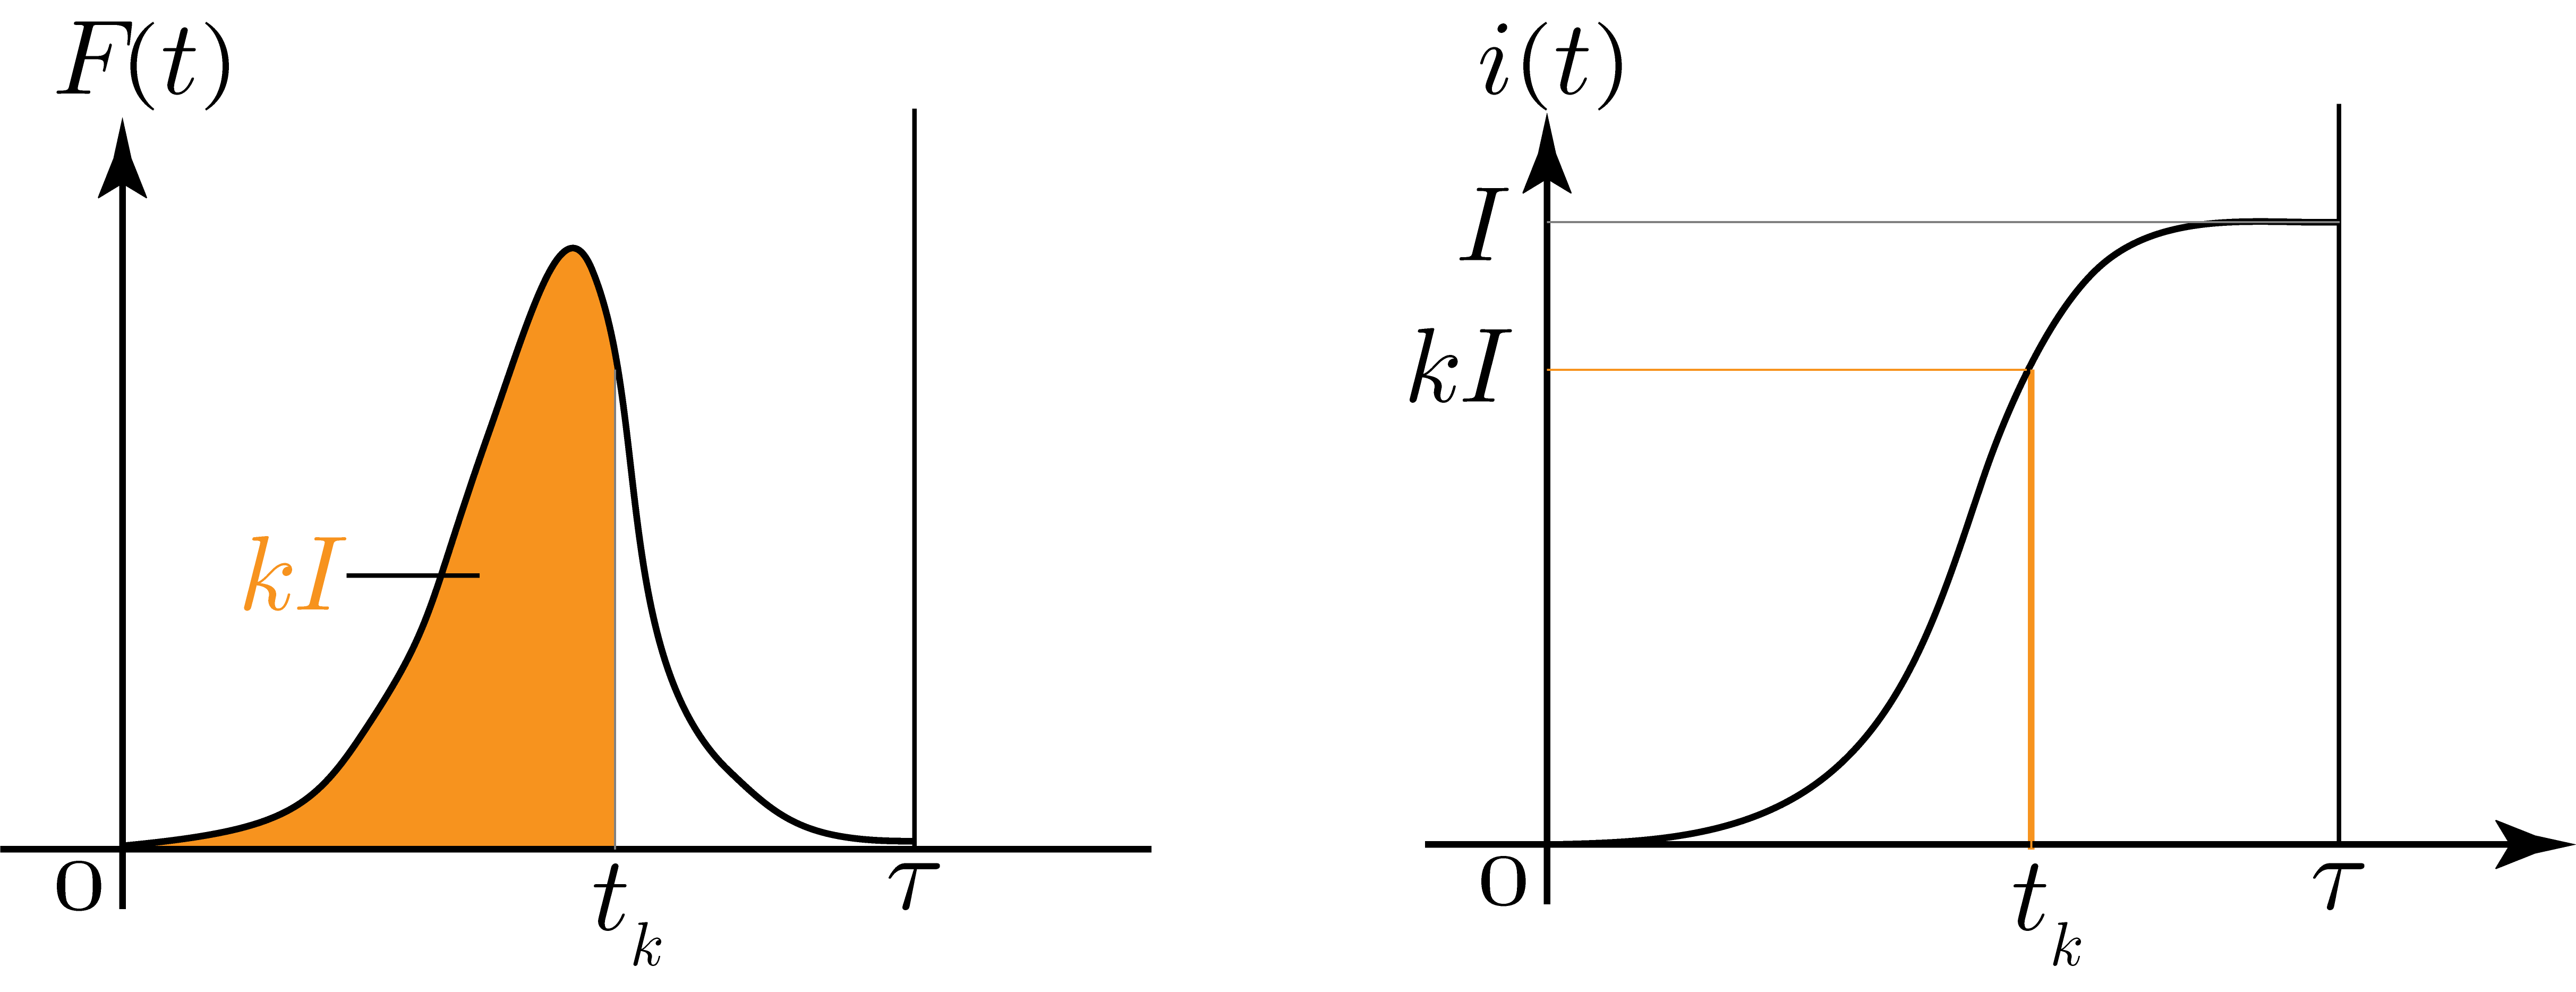
\includegraphics[width=16cm]{image/6-1-12.png}
\caption{力与累积的冲量}
\end{figure}


虽然这个问题倒是也分析地清,\,但这足以告诉我们,\,选取一个简单清晰的模型的必要性.\,为此我们进一步设出碰撞过程中两质点之间持续作用的力$F(t)$,\,它从$0$时刻开始产生到$\tau$时刻作用结束.\,但是,\,并不是只有两质点直接接触才发生作用力,\,事实上我们可以人为把这两个力加在相距较远的两个质点上,\,用这样的模型去等效本来可能复杂的碰撞过程.

我们再把过程中累积的冲量定义为一个函数:
\[i(t)=\int_0^t F(t')\ud t'\]

并且把最终造成的总作用冲量记作$I$:
\[I=\int_0^\tau F(t')\ud t'\]

那就必然有一个时刻冲量累积到$kI$,\,可以把这个时刻记作$t_k$,\,即:
\[i(t_k)=kI\]

事实上由于$i$是严格单调的增函数,\,就存在反函数$i^{-1}$,\,那么这个时间就是:
\[t_k=i^{-1}(kI)\]

有$i^{-1}(0)=0,\,i^{-1}(I)=\tau$.\,这样就足够我们去计算过程中相互作用力的做功了.\,由于是真实碰撞的模拟,\,那么必然$v_1\geq v_2$碰撞才可以发生.\,当冲量累积到$i$时,\,两个质点的速度分别为:
\[u_1=v_1-\frac{i}{m_1}\]
\[u_2=v_2+\frac{i}{m_2}\]

这说明过程$1$速度不断减小,\,$2$速度不断增加.\,现在就足够写出力对$1$和$2$做功的功率了.\,分别为:
\[P_1=-Fu_1=-\frac{\ud i}{\ud t}\left(v_1-\frac{i
}{m_1}\right)\]
\[P_2=Fu_2=\frac{\ud i}{\ud t}\left(v_2+\frac{i
}{m_2}\right)\]

最后如果把功率对时间积分,\,我们发现积分自动以$i$为自变量了:
\[W_1=\int_0^\tau P_1(t)\ud t=-\int_0^I \left(v_1-\frac{i
}{m_1}\right)\ud i\]
\[W_2=\int_0^\tau P_2(t)\ud t=\int_0^I \left(v_2+\frac{i
}{m_2}\right)\ud i\]

线性函数的积分,\,就等于函数值初末值的平均值乘以积分区间的长度,\,这就给出了一个\emph{冲量乘速度形式的功},\,碰撞过程中相互作用力对质点1和质点2的功应当是:
\[W_1=-\frac{1}{2}I(v_1+v_1')\]
\[W_2=\frac{1}{2}I(v_2+v_2')\]

这并不是任何让人意外的结论,\,如果带入动量定理$I=m_1(v_1-v_1')=m_2(v_2'-v_2)$就能发现这两个功无非就是末动能减初动能,\,其实就是反映了动能定律.\,不过注意到表达式推导过程中对动量定律的应用我们发现这个表达式倒不是纯粹的任意情况下都通用的功的定义.\,在使用动量定律前的这个功的积分:
\[W=\int \bs{v}\cdot \ud \bs{I}\]

倒是的确通用的.

如果定义碰前接触速度$v=v_1-v_2$,\,碰后分离速度$v'=v_2'-v_1'$.\,我们可以发现:
\[W_1+W_2=\frac{1}{2}I(v'-v)\]

又定义恢复系数$e=v'/v$.\,碰撞就因此分为四类:

1.\,完全非弹性碰撞,\,$I$最小的情况,\,作为一个实际的碰撞过程分离速度必然也至少为零$v_2'\geq v_1'$,\,否则1仍然在接近2力就不可能会消失.\,所以$I$最小就是让碰撞后共速,\,这样$e=0$就是完全非弹性碰撞的决定$I$大小的条件.

2.\,完全弹性碰撞.\,考虑碰撞过程的能量转化,\,显然,\,如果$W_1+W_2$不等于零,\,前后的总动能就不会是不变量.\,但是如果要求碰前碰后动能不变,\,这就构成了完全弹性碰撞,\,简称弹性碰撞.\,此时,\,除了可以列动能不变来求解$I$,\,我们发现这等价于$v=v'$,\,也就是\emph{接触速度等于分离速度}.\,以后我们将总是认为弹性碰撞的等价对应条件是$e=1$.

3.\,非弹性碰撞(不完全的).\,这是最符合实际情况的一类碰撞.\,这种碰撞中$0<e<1$.\,也就是$v'<v$的情况.\,功$W_1+W_2$是小于零的,\,说明碰撞过程动能有损失,\,能量去向是显而易见的:\,变成了两个碰撞的物体的内能,\,这里的内能可能就是热学上的内能,\,也可以是视作弹性体时虽然整体动量为零但局部有弹性波而产生的宏观动能与势能.\,这种情况之所以普遍是因为,\,碰前往往整个物体没有这样的弹性波,\,能量处于最低的状态,\,碰后这个能量总是会大于零.\,故能量总是有损失的.

4.\,超弹性碰撞.\,也就是$e>1$.\,碰撞后分离速度大于接触速度.\,因碰撞而获得动能.\,这样的过程也并不少见,\,炸弹的爆炸,\,或者刚刚的人推墙使人动起来都是这种情形.\,特点是别的能量会释放出来转化为动能.\,前提需要注意不能违背动量守恒.





\subsection{自由刚体的碰撞}

如果把两个质点的碰撞换为两个自由刚体相碰撞,\,这里我们只考虑平面情况,\,那么同理碰撞会产生一个冲量$\bs{I}$.\,但是这个冲量却有两种可能性,\,如果是光滑的刚体,\,那么碰撞的冲量必然沿法线$n$方向.\,但是如果是粗糙的刚体,\,那么还可以有沿切线方向的分量.\,不管何种情况我们来证明两个恒成立的结论:
\begin{wrapfigure}[14]{o}[-10pt]{6cm}\label{6-1-12}
\centering
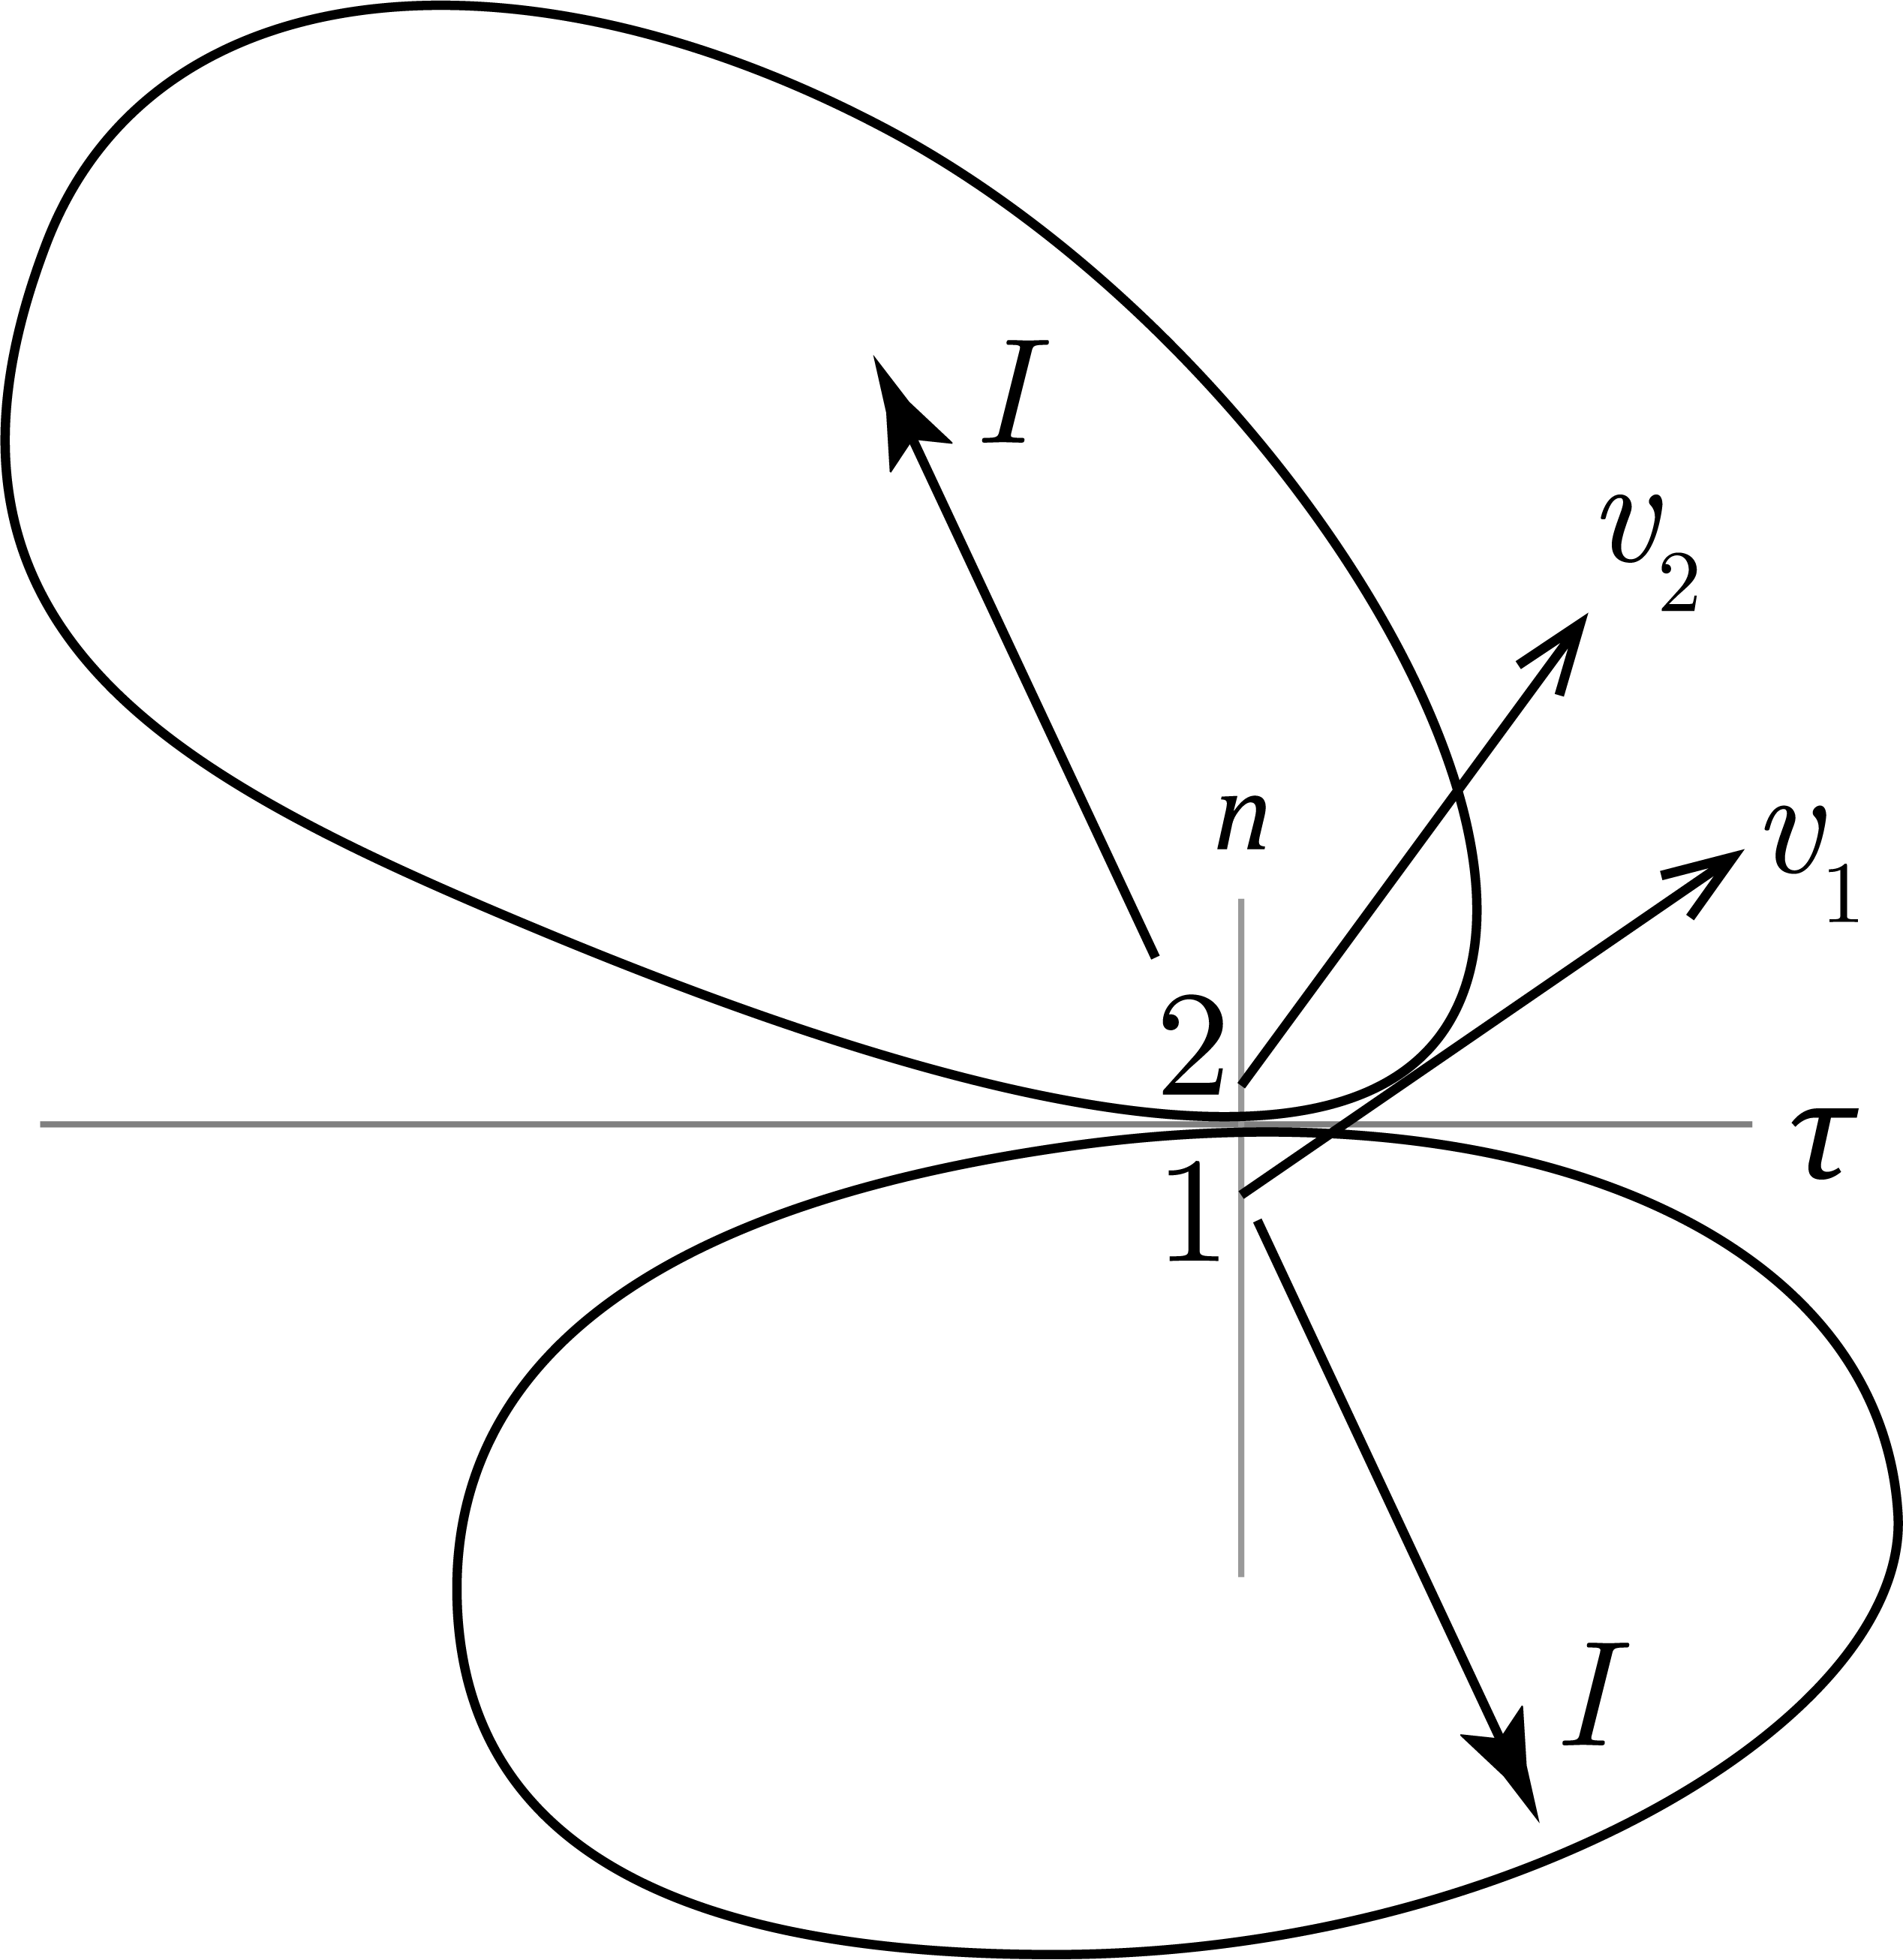
\includegraphics[width=6cm]{image/6-1-13.png}
\caption{两刚体碰撞}
\end{wrapfigure}

一是,\,1对2做的功或2对1做的功总是满足:
\[W=\frac{1}{2}\bs{I}\cdot(\bs{v}+\bs{v}')\]

这里$\bs{v}$和$\bs{v}'$指的便是力的作用点,\,即固连在刚体上的点的速度.\,证明这个定理思路类似于之前的做法.\,我们可以为过程中的冲量累计选取一个变量$k(t)$.\,当$k=0$时碰撞刚刚开始,\,而$k=1$时碰撞就结束了.\,变量取$k$时作用的冲量为:
\[\bs{i}(t)=k(t)\bs{I}\]

那么由于冲量对刚体质心速度和刚体旋转角速度的影响都是线性的,\,而且碰撞点速度也将线性依赖于这些值.\,从而积累到变量$k$时,\,点具有速度:
\[\bs{u}=k\bs{v}'+(1-k)\bs{v}\]

于是利用做功的积分式:
\[W=\int_0^\tau \bs{F}\cdot \bs{u}\ud t=\int_0^{\bs{I}} \bs{u}\cdot \ud \bs{i}=\int_0^1[k\bs{v}'+(1-k)\bs{v}]\cdot\bs{I}\ud k=\frac{1}{2}\bs{I}\cdot(\bs{v}+\bs{v}')\]

二是,\,不损失机械能的条件是,\,或者更特殊地,\,在无摩擦的碰撞中弹性碰撞的条件是,\,接触点形成的沿冲量方向的接触分速度等于该方向的分离分速度.\,这个证明也是简单的.\,只需要把点乘式后面的速度分解在冲量方向并把两个功相加为零即可.\,也就是我们有广义的$e=1$与动能不变作为弹性碰撞的等价条件.


\subsection{多体碰撞}
如果碰撞是多体的往往有两种不同的处理思路:\,一是屡次碰撞的思路,\,最典型的碰撞就是牛顿摆情况,\,小球与多个连续放置的小球的碰撞如果视作屡次的弹性碰撞就能解释体系形成周期性运动的原因.\,因为两个质量相等的小球的碰撞总是简单的交换速度.\,此时我们注意到碰撞结束后,\,最左侧的两球之间从接触速度的$v$变成了$0$,\,而最右侧的两小球却从$0$变成了$v$:
\begin{figure}[H]
\centering
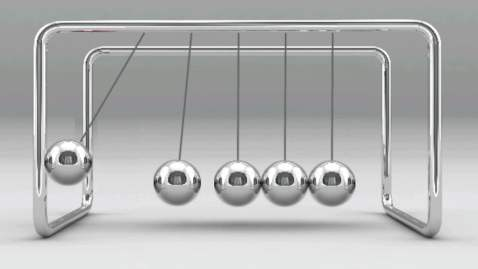
\includegraphics[width=16cm]{image/6-1-14}
\caption{牛顿摆}
\end{figure}

但是如果把最右边的小球要撞击的四个小球视作一个带约束的整体,\,显然既然四个小球必须作为一个整体运动,\,它们之间的相互作用冲量是不会做功的.\,同样的道理也适用于任何带约束的多体碰撞场合,\,虽然碰撞涉及多个物体,\,但是真正具有接触速度的只有一个碰撞点,\,那么作为约束其它点处不可能产生分离速度.\,从而动能不损失的条件依然是在撞击的点处法向接触速度等于分离速度.

不难理解,\,实际的多体碰撞总是介于两种极端情形之间的.\,如果是无限多个无限小的球无限密排,\,这就变成了一个连续的弹性介质中的波动的解的问题,\,波的传播速度和碰撞速度之间的大小关系就成为了一个具有决定性意义的因素.\,容易分析,\,思路一适用与撞击速度很快四个小球还来不及达到平衡的情况.\,而思路二适用于波的传播速度非常快,\,任何冲量作用在四个小球上都相当于在推动四个球构成的整体的情况.

